\section{CONFIGURACIÓN E INSTALACIÓN DE HARDWARE}
\begin{frame}

\pgfdeclareimage[width=\paperwidth,height=\paperheight]{bg}{imagenes/fondo_seccion}
\setbeamertemplate{background}{\pgfuseimage{bg}}

\definecolor{greenU}{RGB}{212,202,72}
\setbeamercolor{block body}{fg=Black,bg=greenU}
\begin{block}{}
\centering
\vspace{8mm}
\Large{CONFIGURACIÓN E INSTALACIÓN DE HARDWARE}
\vspace{8mm}
\end{block}
\end{frame}
%-----------------------

{
\begin{frame}
\frametitle{Parte II - Tabla de contenidos}
\begin{spacing}{1.5}
\tableofcontents[currentsection,sectionstyle=hide/hide,subsectionstyle=show/show/hide, subsubsectionstyle=hide]
\end{spacing}
\end{frame}
}


\subsection{Lab6: RTL}
%*********************
\begin{frame}{}

\pgfdeclareimage[width=\paperwidth,height=\paperheight]{bg}{imagenes/fondo_lab}
\setbeamertemplate{background}{\pgfuseimage{bg}}

\bfseries{\textrm{\LARGE Lab6\\ \Large RTL}}
\raggedright
\end{frame}
%*********************

\begin{frame}{RTL\_SDR}

\pgfdeclareimage[width=\paperwidth,height=\paperheight]{bg}{imagenes/fondo3}
\setbeamertemplate{background}{\pgfuseimage{bg}}


El RTL\_SDR es un dispositivo el cual permite combinar tanto la parte de software como hardware para implementar un sistema con el cual sea posible desarrollar procesos de radiocomunicaciones tanto de recepción como de transmisión de señales.\\ \vspace{2mm}
El RTL se creó principalmente para solucionar los problemas de compilación para equipos con procesamiento de Pentium 4, esta tarjeta está diseñada para poder demodular señales en FM, AM y SSB con diferentes anchos de banda; también tiene la capacidad de analizar más de cien frecuencias en un segundo.\\\vspace{2mm}
En general el RTL es una gran ayuda a nivel educativo ya que ayuda a hacer una estación receptora si no se tiene una.


\end{frame}
%----------------
\begin{frame}{Instalación de paquetes}

En la siguiente guía práctica se dará un ejemplo por medio de uso de terminal y órdenes, para la captura de señales de radio FM, escáner de la policía, airband scanner y decodificador de localización.

\end{frame}
%------------------------

\begin{frame}
\frametitle{Instalación de Paquetes}

Para instalar los paquetes desde consola se debe ingresar las siguientes órdenes.

\textbf{Paquetes de SOX}
\begin{itemize}
 
    \item { Mediante esta órden, es posible la descarga de las librerías o paquetes necesarios para el correcto y completo funcionamiento de SOX.
    \begin{block}{}
    \texttt
    {\ \ \ root@user\~\$ sudo apt-get install libsox-fmt-alsa}
    \end{block}}
    
    \item{Este paquete contiene la mayoría de las bibliotecas de formatos de audio compatibles con SOX
    \begin{block}{}
    \texttt
    {\ \ \ root@user\~\$ sudo apt-get install libsox-fmt-base}
    \end{block}}
\end{itemize}

\end{frame}
%--------------------------

\begin{frame}
\frametitle{Instalación de Paquetes}

\begin{itemize}
    \item {Este paquete contiene la biblioteca sox que permite convertir varios formatos de archivos de audio de computadora en otros formatos.
    \begin{block}{}
    \texttt
    {\ \ \ root@user\~\$ sudo apt-get install libsox2}
    \end{block}}
    
    \item{SOX es una herramienta conocida como “la navaja suiza” en manipulación de audio, ya que contiene las bibliotecas I/O que permiten el procesamiento del audio en diversos formatos.
    \begin{block}{}
    \texttt
    {\ \ \ root@user\~\$ sudo apt-get install sox}
    \end{block}}
\end{itemize}

\end{frame}
%--------------------------

\begin{frame}
\frametitle{Instalación de Paquetes}

\begin{itemize}
    \item {Este paquete contiene una biblioteca compartida.
    \begin{block}{}
    \texttt
    {\ \ \ root@user\~\$ sudo apt-get install libgnuradio-osmosdr0.1.4}
    \end{block}}
    
    \item{Este paquete es el software que proporciona el control del hardware USB e independientemente de la API, pasar datos a aplicaciones de radio definidas por software en el host. Tiene la posibilidad de recibir o transmitir información.
    \begin{block}{}
    \texttt
    {\ \ \ root@user\~\$ sudo apt-get install libosmosdr0}
    \end{block}}
\end{itemize}

\end{frame}
%--------------------------

\begin{frame}
\frametitle{Instalación de Paquetes}
\textbf{Paquetes de RTL\_SDR}
\begin{itemize}
 
    \item { Es un software que soporta dispositivos SDR tales como Airspy, funcube Dongles, rtl-sdr, HackRF, y USRP
    \begin{block}{}
    \texttt
    {\ \ \ root@user\~\$ sudo apt-get install gqrx-sdr}
    \end{block}}
     \item { Este archivo contiene librerías y archivos de desarrollo que complemetan el funcionamiento de conexión de la RTL.
    \begin{block}{}
    \texttt
    {\ \ \ root@user\~\$ sudo apt-get install librtlsdr-dev}
    \end{block}}
\end{itemize}

\end{frame}
%--------------------------

\begin{frame}
\frametitle{Instalación de Paquetes}
\begin{itemize}
 
    \item {Este paquete contiene una biblioteca compartida.
    \begin{block}{}
    \texttt
    {\ \ \ root@user\~\$ sudo apt-get install librtlsdr0}
    \end{block}}
    \item {Este paquete permite el recepcionamiento I/Q para dispositivos basados en la RTL2832. 
    \begin{block}{}
    \texttt
    {\ \ \ root@user\~\$ sudo apt-get install rtl-sdr}
    \end{block}}
\end{itemize}

\end{frame}
%--------------------------

\begin{frame}
\frametitle{Procedimiento}

Para iniciar es necesario abrir una nueva terminal, desde allí se realizará el procedimiento para comprobar la conexión del hardware RTL con su computadora. \vspace{2mm}
Se debe ingresar la siguiente orden:

\begin{block}{}
    \texttt
    {\ \ \ root@user\~\$ rtl\_test}
    \end{block}

\texttt{rtl\_test} es una herramienta verificadora de la conexión para receptores DVB-T basados en RTL2832. \\ \vspace{2mm}
Si existe una respuesta satisfactoria evidenciará el siguiente mensaje:

\begin{block}{}
    \texttt
    {Info: This tool will continuously read from the device, and report if samples get lost. If you observe no further output, everything is fine. Reading samples in async mode... cb transfer status: 1, canceling...}
    \end{block}

\end{frame}
%--------------------------

\begin{frame}
\frametitle{Procedimiento}

Si el hadware RTL no está conectado evidenciará el siguiente mensaje:

\begin{block}{}
    \texttt
    {No supported devices found.}
    \end{block}

Al conectar mas de un dispositivo RTL y ejecutar la orden \texttt{rtl\_test}, se visualiza un listado de los dispositivos con sus respectivas referencias, como se muestra a continuación.
    
    \begin{block}{}
    \texttt
    {Found 2 device(s):\\
    0:  Realtek, RTL2838UHIDIR, SN: 00000001\\ 
    1:  Realtek, RTL2838UHIDIR, SN: 00000001\\
    Using device 0: Generic RTL2832U OEM\\ 
    Found Rafael Micro R820T tuner\\ 
    Supported gain values (29): 0.0 0.9 1.4 2.7 3.7 7.7 8.7 12.5 14.4 15.7 16.6 19.7 20.7 22.9 25.4 28.0 29.7 32.8 33.8 36.4 37.2 38.6 40.2 42.1 43.4 43.9 44.5 48.0 49.6\\
    {[R82XX]} PLL not locked!\\
    Sampling at 2048000 S/s. 
}
    \end{block}

\end{frame}
%--------------------------

\begin{frame}
\frametitle{Procedimiento}

Al ser desconectada la RTL mientras se ejecuta el test lo notifica mediante el siguiente mensaje: 

\begin{block}{}
    \texttt{
    Reading samples in async mode... \\
    lost at least 84 bytes \\
    cb transfer status: 5, canceling... \\
    cb transfer status: 5, canceling... \\
    cb transfer status: 5, canceling... \\
    cb transfer status: 5, canceling... \\
    cb transfer status: 5, canceling... \\\vspace{2mm}
    Library error -5, exiting…\\}
\end{block}

\end{frame}
%--------------------------

\begin{frame}
\frametitle{Procedimiento}

\textbf{Receptor de Radio Pública FM}\\
\vspace{2mm}
Para esta práctica se debe realizar desde la terminal, puede utilizar la misma o abrir una nueva. Se ingresa la siguiente órden:

\begin{block}{}
  \texttt{
  \ \ \ root@user\~\$ rtl\_fm -M wbfm -f 103.3M -s 1000k -l 0
    \begin{itemize}
      \item[] {|play -r 32k -t raw -e s -b 16 -c 1 -V1 -}
    \end{itemize}}
\end{block} 

\end{frame}
%--------------------------

\begin{frame}
\frametitle{Procedimiento}

En donde cada uno de los componentes del mando \texttt{rtl\_fm} , tienen una función especifica para poder captar la señal de radio FM.

\begin{itemize}
    \item {\textit{-f 103.3M : } Indica la frecuencia de sintonización, es decir la de la Radio Pública a escuchar, para este caso 103.3MHz.}
    \item {\textit{-M wbfm :} Define el tipo de modulación, WBFM (banda ancha).Por defecto es fm (NBFM).Las opciones para -M son, fm, wbfm, raw, am, usb, lsb.}
    \item {\textit{-s 1000k :} Indica que se toma una tasa de muestreo de 1MS/s}
    \item {\textit{-l 0 :} Deshabilita el squelch (actúa para suprimir la salida de audio de un receptor en ausencia de una señal de entrada deseada suficientemente fuerte)}
\end{itemize}

\end{frame}
%--------------------------

\begin{frame}
\frametitle{Procedimiento}

Para ver más opciones de \texttt{rtl\_fm}, ejecute lo siguiente::

\begin{block}{}
  \texttt{
  \ \ \ root@user\~\$ rtl\_fm --help}
\end{block} 

Ahora bien, se utiliza el caracter \textbar  \ el cual es un conector para relacionar la orden \texttt{rtl\_fm} con la orden \texttt{play} para poder escuchar en el computador, la emisora sintonizada.

\begin{block}{}
  \texttt{
  \ \ \ root@user\~\$ rtl\_fm... |play -r 32k -t raw -e s -b 16 -c 1
    \begin{itemize}
      \item[] {-V1 -}
    \end{itemize}}
\end{block} 

\end{frame}
%--------------------------

\begin{frame}
\frametitle{Procedimiento}

\texttt{play} es un reproductor que lee y escribe archivos de audio en los formatos más populares y opcionalmente puede aplicarles efectos. Puede combinar múltiples fuentes de entrada, sintetizar audio y, en muchos sistemas, actuar como un reproductor de audio de propósito general o un grabador de audio multimedia. \\
\vspace{2mm }
Cada uno de los componentes de play, tiene una función específica, para la reproducción de la señal captada:

\begin{itemize}
    \item {\textit{-r : } Usa números aleatorios por defecto (lo mismo en cada ejecución de SOX)}
    \item {\textit{-t : } Tipo de archivo de audio FILETYPE}
    \item {\textit{-s : } Muestra el progreso mientras procesa los datos de audio fuerte)}
    \item {\textit{-b : } BITS Tamaño de muestra codificado en bits}
    \item {\textit{-c : } Factor de compresión para formato de salida}
    \item {\textit{-v : } Factor de ajuste del volumen del archivo de entrada (número real)}
    \item {\textit{raw : } Enlaza un dispositivo de caracteres brutos de Linux}
\end{itemize}


\end{frame}
%--------------------------

\begin{frame}
\frametitle{Procedimiento}

Para ver más opciones de play, ejecute lo siguiente:

\begin{block}{}
  \texttt{
  \ \ \ root@user\~\$ Play {-}help}
\end{block} 

Finalmente, se obtendrá una respuesta, en donde se podrá visualizar la recepción de radio FM y escuchar la emisora sintonizada.

\end{frame}
%--------------------------

\begin{frame}
\frametitle{Procedimiento}

Adicionalmente se realizó una prueba simple de las órdenes instaladas, en el software GNU Radio, implementando un transmisor FM.  

\begin{center}
\vspace{-0.3cm}
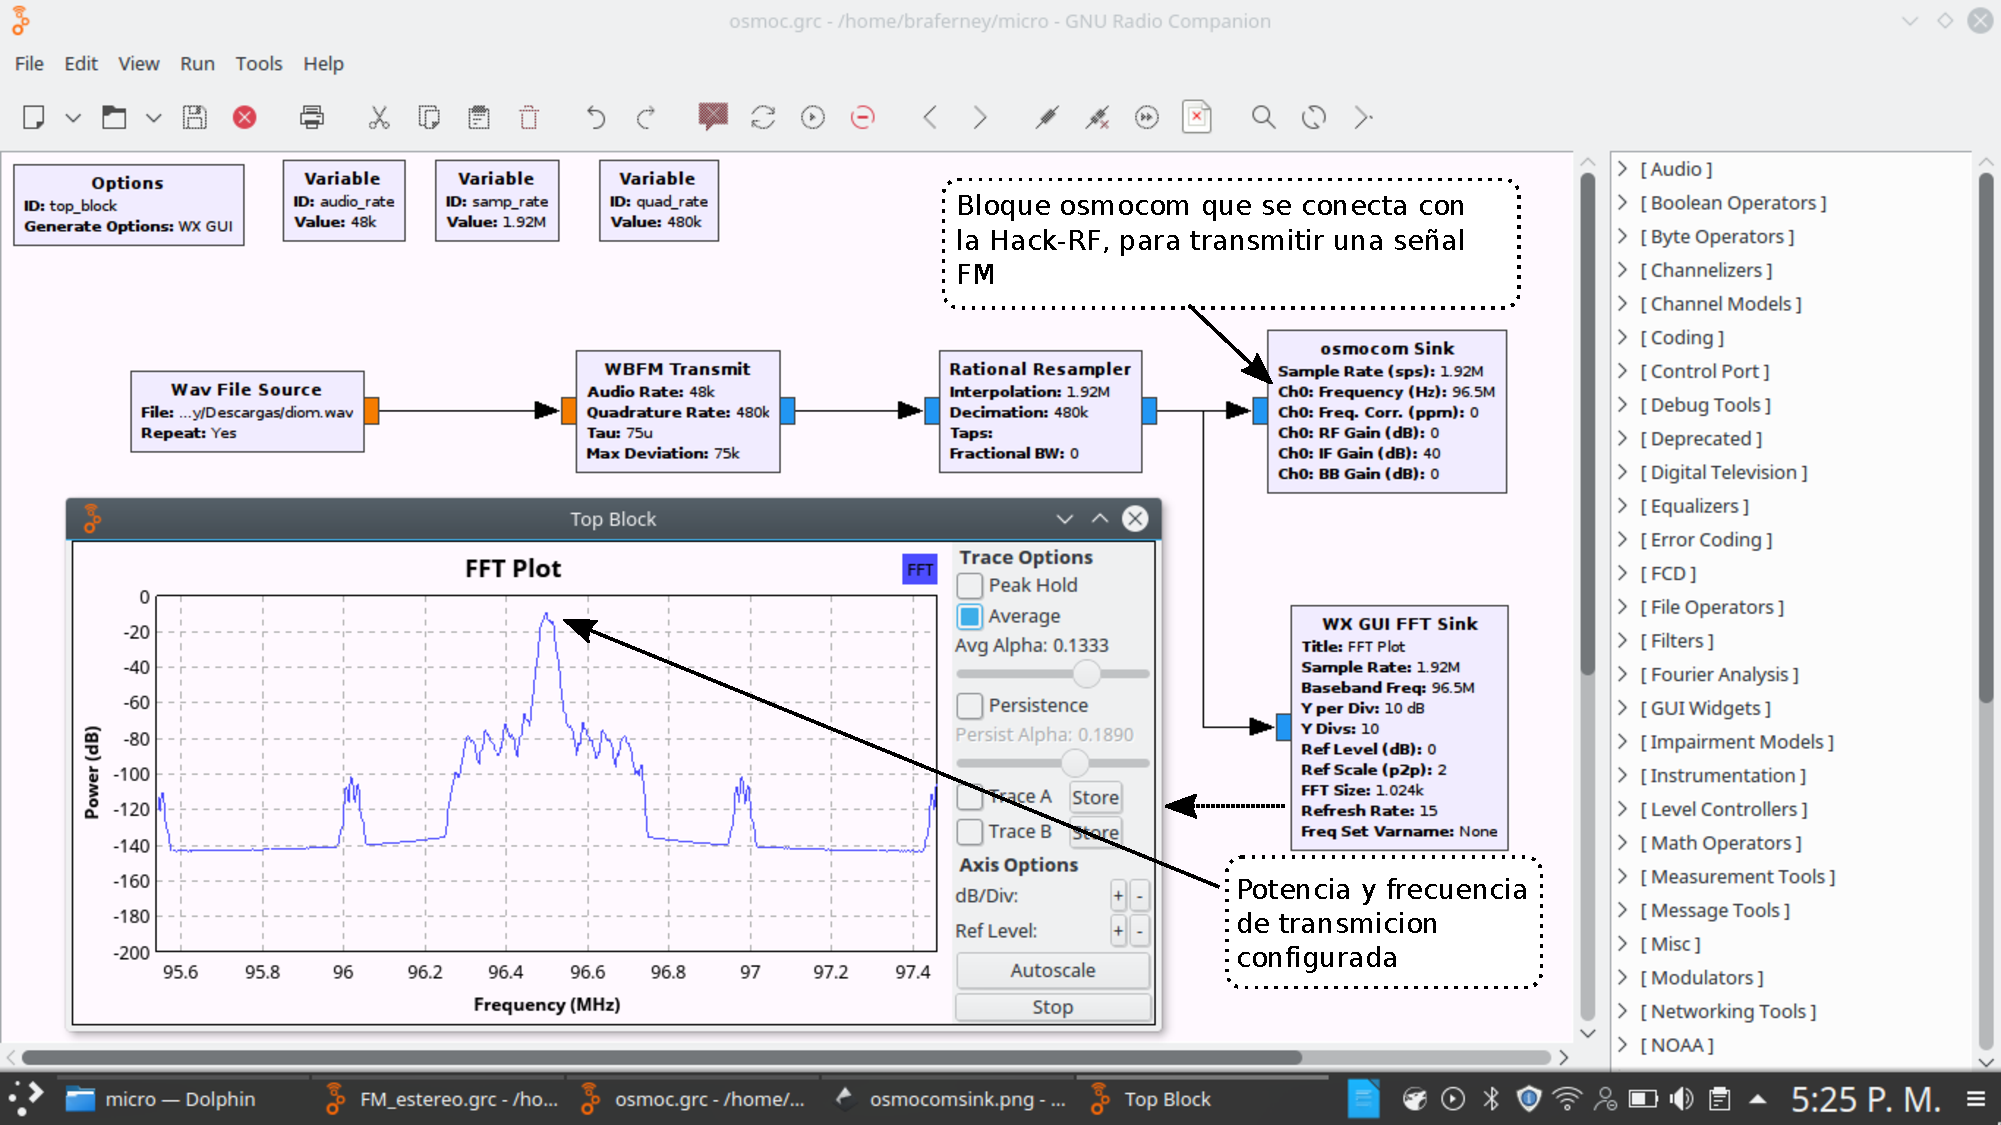
\includegraphics[width=\textwidth]{parte2/lab6/pdf/lab6_1.pdf}
\end{center}


\end{frame}
%--------------------------

%///////////////////////////////////////////////////////////////

\subsection{Lab7: HackRF One}
%*********************
\begin{frame}{}

\pgfdeclareimage[width=\paperwidth,height=\paperheight]{bg}{imagenes/fondo_lab}
\setbeamertemplate{background}{\pgfuseimage{bg}}

\bfseries{\textrm{\LARGE Lab7\\ \Large HackRF One}}
\raggedright
\end{frame}
%*********************

\begin{frame}{HackRF One}

\pgfdeclareimage[width=\paperwidth,height=\paperheight]{bg}{imagenes/fondo3}
\setbeamertemplate{background}{\pgfuseimage{bg}}


HackRF One es un periférico SDR capaz de transmitir o recibir señales de radio desde 1 MHz hasta 6 GHz, fabricado por Great Scott Gadgets. Fue diseñado para facilitar el  desarrollo para las nuevas generaciones de tecnologías radio y sus correspondientes protocolos. Es un transceiver con capacidad de operación half-duplex .  Tiene una capacidad de muestreo de hasta 20 millones de muestras por segundo, pudiéndose alcanzar las 21,5 en función del tipo de controlador USB 2.0 HS que incluya el computador al que se conecta

\end{frame}
%-----------------------------------

\begin{frame}{Características}

\begin{center}
\vspace{-0.3cm}
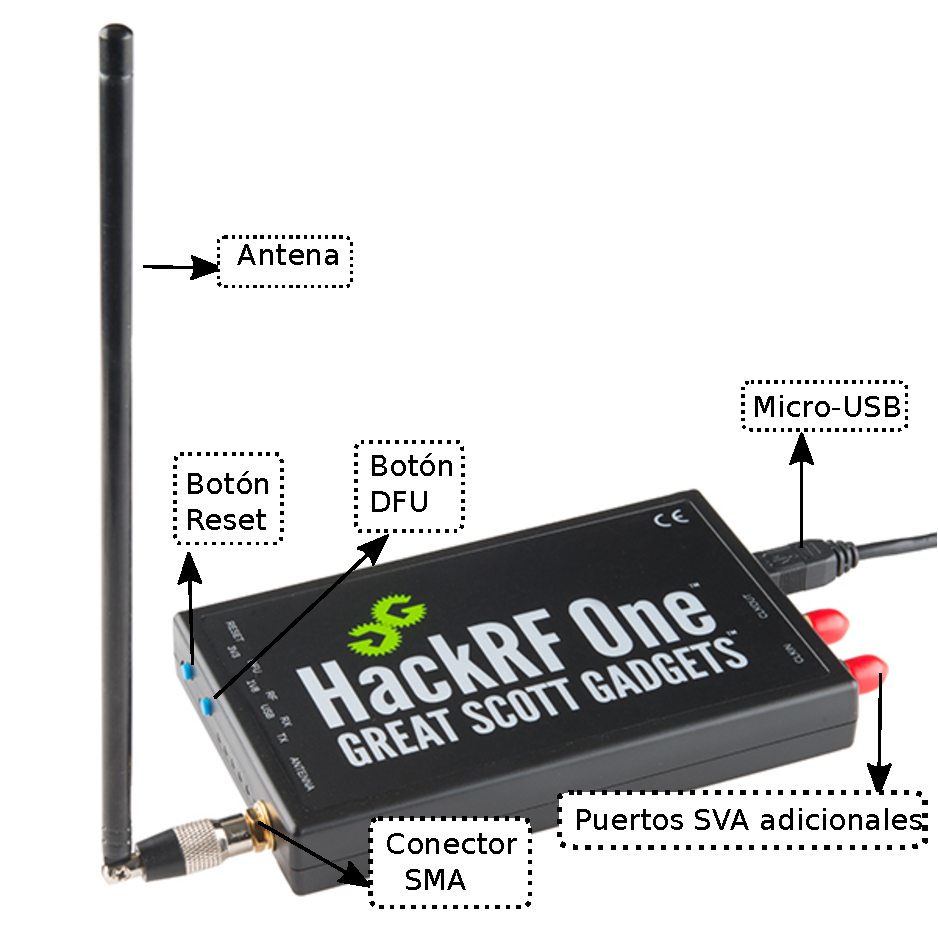
\includegraphics[width=.7\textwidth]{parte2/lab7/pdf/lab7_1.pdf}
\end{center}

\end{frame}
%-----------------------------------

\begin{frame}{Instalación de  herramientas de la HackRF One}

\begin{itemize}
    \item
    {Conecte el HackRF One a la computadora con el cable Micro-USB a USB. Confirme que los primeros tres  LEDs se iluminan para asegurar que el dispositivo esté funcionando.}
    \item
    {Las bibliotecas se pueden instalar con la siguiente órden en la terminal:
    
    \begin{block}{}
    \texttt{
    sudo apt-get install hackrf}
    \end{block}
    }
    \item
    {Después de la instalación, digite la orden "hackrf\_info" para verificar que el dispositivo HRF1 esté conectado.}
    
\end{itemize}
\end{frame}
%-----------------------------------

\begin{frame}{Instalación de  herramientas de la HackRF One}

\begin{itemize}
    \item
    {Estas son algunas herramientas utilizadas en HackRF One:
    \begin{itemize}
        \item  {\textit{hackrf\_info :} permite al usuario probar el dispositivo y mostrar la configuración.}
        \item  {\textit{hackrf\_max2837 :} permite al usuario controlar el chip max2837}
        \item  {\textit{hackrf\_spiflash :} permite al usuario configurar el Flash incorporado.}
        \item  {\textit{hackrf\_transfer :} permite al usuario recibir datos de RF y transmitir datos a RF.}
        \item  {\textit{hackrf\_si5351c :} permite al usuario controlar el chip si5351c.}
        \item  {\textit{hackrf\_cpldjtag :} permite al usuario configurar el CPLD integrado.}
    \end{itemize}
    }
\end{itemize}
\end{frame}
%-----------------------------------

\begin{frame}{Instalación de  herramientas de la HackRF One}

\begin{itemize}
    \item
    {Después de una instalación exitosa, la terminal debe responder con: \hspace{1pt} \ttfamily{found hackrf board}}
    \item
    {Si la terminal muestra que la HRF1 no está conectada, solucione los problemas verificando que los cables estén enchufados y se está suministrando potencia al dispositivo}
    
\end{itemize}
\end{frame}
%-----------------------------------

\begin{frame}{Actualización del firmware}

\begin{itemize}
    \item [Paso 1]
    {\textbf {Actualizar el firmware de SPI Flash }\\ Para actualizar el firmware en un HackRF One que funcione, use el programa \texttt{hackrf\_spiflash}:
    
    \begin{block}{}
    \texttt{
    hackrf\_spiflash -w hackrf\_one\_usb.bin}
    \end{block}
    
    Puede encontrar el firmware binario (hackrf\_one\_usb.bin) en el directorio firmware-bin del último paquete de versiones o puede compilar el suyo desde la fuente. Para Jawbreaker, use hackrf\_jawbreaker\_usb.bin. Si compila desde el origen, el archivo se llamará hackrf\_usb.bin. 
    }
    
\end{itemize}
\end{frame}
%-----------------------------------

\begin{frame}{Actualización del firmware}

\begin{itemize}
    \item [Paso 2]
    {\textbf {Actualizar el CPLD}\\ Para actualizar a la última imagen CPLD, primero actualice el firmware SPI flash, libhackrf y hackrf-tools. Entonces en la terminal se ingresa lo siguiente:
    
    \begin{block}{}
    \texttt{
    hackrf\_cpldjtag -x firmware / cpld / sgpio\_if / default.xsvf}
    \end{block}
    
    Después de unos segundos, tres LEDs deberían comenzar a parpadear. Esto indica que el CPLD se ha programado con éxito. Restablezca el dispositivo HackRF presionando el botón RESET o desenchufando y enchufando de nuevo.
    }
    
\end{itemize}
\end{frame}
%-----------------------------------

\begin{frame}{Instalación de paquetes para trabajar con GNU Radio: osmocom}

A continuación instalamos los paquetes de osmocom.

\begin{block}{}
    \texttt{
    \ \ \ git clone git://git.osmocom.org/gr-osmosdr}
\end{block}

Nos movemos dentro de la carpeta clonada:

\begin{block}{}
    \texttt
    {\ \ \ cd gr-osmosdr}
\end{block}


Creamos el directorio de construcción, nos movemos dentro y hacemos el cmake.

\begin{block}{}
  \texttt{
  \ \ \ mkdir build \&\& cd build
    \begin{itemize}
      \item[] cmake ../
    \end{itemize}}
\end{block}  
\end{frame}
%-----------------------------------

\begin{frame}{Instalación de paquetes para trabajar con GNU Radio: osmocom}
Construimos e instalamos.

\begin{block}{}
  \texttt{
  \ \ \ make
    \begin{itemize}
      \item[] sudo make install
      \item[]  sudo ldconfig
    \end{itemize}}
\end{block}  

\end{frame}
%-----------------------------------

\begin{frame}{Ejemplo mínimo}
    \begin{center}
    \vspace{-0.3cm}
    imagen que no ha sido enviada
    %\includegraphics[width=\textwidth]{parte2/lab7/pdf/lab7_4.pdf}
    \end{center}
\end{frame}






